% !TeX program = xelatex
\documentclass[a4paper,10pt]{article}

% ============================================================================
% ១. កញ្ចប់បណ្ណាល័យ និងការកំណត់ទំព័រ (Packages & Page Setup — តាមគំរូ ls_plan.tex)
% ============================================================================
\usepackage[a4paper, left=0.95cm, right=0.95cm, top=0.85cm, bottom=0.92cm, footskip=0.52cm]{geometry}
\usepackage{amsmath}
\usepackage{unicode-math}
\usepackage{fontspec}
\usepackage{longtable, array, multirow, colortbl}
\usepackage[table]{xcolor}
\usepackage{enumitem}
\usepackage{pifont}
\usepackage{fancyhdr}
\usepackage{tikz}
\usetikzlibrary{calc, arrows.meta, decorations.pathreplacing, patterns, positioning, babel}

\makeatletter
\let\@expl@@@mark@update@singlecol@structures@@\relax
\makeatother

% --- ប្រព័ន្ធស្វែងរកទីតាំងពុម្ពអក្សរស្វ័យប្រវត្តិ (Windows Local + Cloud Repo fonts/) ---
\providecommand{\NGSFindFonts}{%
  \IfFileExists{C:/Windows/Fonts/cambria.ttc}{%
    \def\NGSSysPath{C:/Windows/Fonts/}%
    \def\NGSUserPath{C:/Users/KIT/AppData/Local/Microsoft/Windows/Fonts/}%
  }{%
    \IfFileExists{./fonts/KhmerOSsiemreap.ttf}{\def\NGSSysPath{./fonts/}\def\NGSUserPath{./fonts/}}{%
    \IfFileExists{../fonts/KhmerOSsiemreap.ttf}{\def\NGSSysPath{../fonts/}\def\NGSUserPath{../fonts/}}{%
    \IfFileExists{../../fonts/KhmerOSsiemreap.ttf}{\def\NGSSysPath{../../fonts/}\def\NGSUserPath{../../fonts/}}{%
    \IfFileExists{../../../fonts/KhmerOSsiemreap.ttf}{\def\NGSSysPath{../../../fonts/}\def\NGSUserPath{../../../fonts/}}{%
    \IfFileExists{../../../../fonts/KhmerOSsiemreap.ttf}{\def\NGSSysPath{../../../../fonts/}\def\NGSUserPath{../../../../fonts/}}{%
    \IfFileExists{../../../../../fonts/KhmerOSsiemreap.ttf}{\def\NGSSysPath{../../../../../fonts/}\def\NGSUserPath{../../../../../fonts/}}{%
    \IfFileExists{../../../../../../fonts/KhmerOSsiemreap.ttf}{\def\NGSSysPath{../../../../../../fonts/}\def\NGSUserPath{../../../../../../fonts/}}{%
      \def\NGSSysPath{../../../../../../../fonts/}\def\NGSUserPath{../../../../../../../fonts/}%
    }}}}}}}%
  }%
}
\NGSFindFonts

% ============================================================================
% ២. កំណត់ពុម្ពអក្សរ (Fonts — តាមគំរូ ls_plan.tex)
% ============================================================================
\setmathfont[Path={\NGSSysPath}, FontIndex=1, Scale=1.02]{cambria.ttc}
\defaultfontfeatures{Ligatures=TeX}

\setmainfont[
  Path={\NGSUserPath},
  Extension=.ttf,
  Script=Khmer,
  BoldFont={KhmerOSsiemreap},
  BoldFeatures={FakeBold=1.8},
  ItalicFont={KhmerOSsiemreap},
  ItalicFeatures={FakeSlant=0.25},
  BoldItalicFont={KhmerOSsiemreap},
  BoldItalicFeatures={FakeBold=1.8, FakeSlant=0.25}
]{KhmerOSsiemreap}

\newfontfamily\muol[Path={\NGSUserPath}, Extension=.ttf, Script=Khmer]{KhmerOSmuollight}
\newfontfamily\Tacteing[Path={\NGSUserPath}, Extension=.TTF]{TACTENG}
\newfontfamily\TimesEn[Path={\NGSSysPath}, Extension=.ttf, BoldFont={timesbd}, ItalicFont={timesi}, BoldItalicFont={timesbi}]{times}
\newfontfamily\CalibriFont[Path={\NGSSysPath}, Extension=.ttf]{calibri}
\newfontfamily\CourierCirc[Path={\NGSSysPath}, Extension=.ttf]{cour}

\XeTeXlinebreaklocale "km"
\XeTeXlinebreakskip = 0pt plus 1pt minus 0.1pt

% ============================================================================
% ៣. ពណ៌ និងការតុបតែង (Colors & Styles)
% ============================================================================
\definecolor{stepbg}{HTML}{D9D9D9}
\definecolor{headgray}{HTML}{E6E6E6}
\definecolor{emphred}{HTML}{C00000}

\pagestyle{fancy}
\fancyhf{}
\renewcommand{\headrulewidth}{0pt}
\fancyfoot[R]{\CalibriFont\fontsize{9pt}{11pt}\selectfont\thepage}

\setlength{\parindent}{0pt}
\setlength{\parskip}{0pt}
\setlength{\tabcolsep}{4.5pt}
\setlength{\LTpre}{2pt}
\setlength{\LTpost}{2pt}

\newcolumntype{L}[1]{>{\raggedright\arraybackslash}p{#1}}
\newcolumntype{C}[1]{>{\centering\arraybackslash}p{#1}}

% ============================================================================
% ៤. ពាក្យបញ្ជាជំនួយ (Helper Macros)
% ============================================================================
\newcommand{\en}[1]{{\TimesEn #1}}
\newcommand{\enbf}[1]{{\TimesEn\bfseries #1}}
\newcommand{\khmflourish}{{\Tacteing\fontsize{15pt}{15pt}\selectfont 3}}
\newcommand{\wcirc}{{\CourierCirc\fontsize{9.5pt}{11pt}\selectfont o}}
\newcommand{\ditem}{{\fontsize{7.5pt}{10pt}\selectfont\ding{117}}\ }
\newcommand{\fiveE}[1]{\textcolor{emphred}{\CalibriFont\bfseries #1}}
\newcommand{\redsub}[1]{\textcolor{emphred}{#1}}
\newcommand{\timenote}[1]{\textcolor{emphred}{\textit{#1}}}
\newcommand{\stepheader}[1]{\multicolumn{3}{|c|}{\cellcolor{stepbg}\muol #1} \\ \hline}
\newcommand{\cfig}[1]{{\centering\vspace{3pt}#1\vspace{3pt}\par}}
\newcommand{\cnum}[1]{\mbox{\fontsize{10.5pt}{12pt}\selectfont\ding{\numexpr181+#1\relax}}}
\newcommand{\unit}[1]{\,\text{\en{#1}}}
\newcommand{\riel}{\,\text{៛}}
\newcommand{\graybox}[1]{\colorbox{headgray}{\strut #1}}

% ============================================================================
% ៥. រូបភាព TikZ ស-ខ្មៅ សម្រាប់បង្រៀនលើក្ដារខៀន និងសន្លឹកកិច្ចការ (B&W Diagrams)
% ============================================================================

% ១. E1 Engage: បេសកកម្មជាងអគ្គិសនីវាស់មុខកាត់ការេជ្រុង 1 mm = 10^{-3} m
\newcommand{\figEngageMEASFourOne}{%
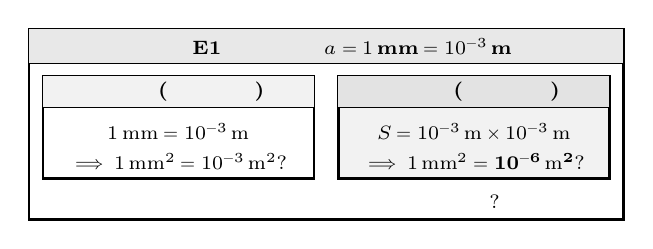
\begin{tikzpicture}[x=1cm, y=1cm, every node/.style={font=\scriptsize, text=black}]
  \draw[black, line width=0.9pt] (0,0) rectangle (7.55,2.42);
  \fill[gray!18] (0,1.98) rectangle (7.55,2.42);
  \draw[black, line width=0.6pt] (0,1.98) -- (7.55,1.98);
  \node at (3.775,2.20) {\textbf{បេសកកម្ម \en{E1}៖ ការេតូចមានជ្រុង $a = 1\unit{mm} = 10^{-3}\unit{m}$}};

  % Left: Apprentice 1 (Linear misconception)
  \draw[black, line width=0.8pt] (0.18,0.52) rectangle (3.62,1.82);
  \fill[gray!10] (0.18,1.42) rectangle (3.62,1.82);
  \draw[black, line width=0.5pt] (0.18,1.42) -- (3.62,1.42);
  \node at (1.90,1.62) {\textbf{កូនជាងទី ១ (បំប្លែងតាមប្រវែង)}};
  \node at (1.90,1.12) {$1\unit{mm} = 10^{-3}\unit{m}$};
  \node at (1.90,0.74) {$\implies 1\unit{mm}^2 = 10^{-3}\unit{m}^2$?};

  % Right: Apprentice 2 (Squared truth)
  \draw[black, line width=0.95pt, fill=gray!10] (3.93,0.52) rectangle (7.37,1.82);
  \fill[gray!22] (3.93,1.42) rectangle (7.37,1.82);
  \draw[black, line width=0.55pt] (3.93,1.42) -- (7.37,1.42);
  \node at (5.65,1.62) {\textbf{កូនជាងទី ២ (គុណជ្រុងនឹងជ្រុង)}};
  \node at (5.65,1.12) {$S = 10^{-3}\unit{m} \times 10^{-3}\unit{m}$};
  \node at (5.65,0.74) {$\implies 1\unit{mm}^2 = \mathbf{10^{-6}\unit{m}^2}$?};

  \node at (3.775,0.23) {\textbf{សំណួរគន្លឹះ៖} តើស្វ័យគុណខ្នាតផ្ទៃក្រឡា ត្រូវរក្សាដដែល ឬលើកការេ?};
\end{tikzpicture}}

% ២. E2 Explore: មុខកាត់ខ្សែភ្លើងរាងស៊ីឡាំង (គំរូទី ១៖ d = 2 mm = 2 x 10^{-3} m)
\newcommand{\figWireCrossMEASFourOne}{%
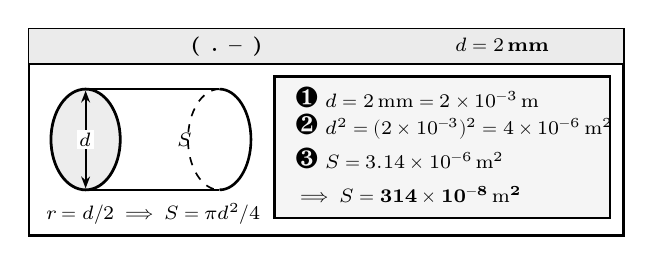
\begin{tikzpicture}[x=1cm, y=1cm, every node/.style={font=\scriptsize, text=black}]
  \draw[black, line width=0.9pt] (0,0) rectangle (7.55,2.62);
  \fill[gray!16] (0,2.18) rectangle (7.55,2.62);
  \draw[black, line width=0.6pt] (0,2.18) -- (7.55,2.18);
  \node at (3.775,2.40) {\textbf{លំហាត់គំរូទី ១ (ទំ.៤៣--៤៤)៖ ខ្សែភ្លើងរាងស៊ីឡាំង អង្កត់ផ្ចិត $d = 2\unit{mm}$}};

  % Cylinder wire drawing on left
  \fill[gray!14] (0.72,1.22) ellipse (0.44cm and 0.64cm);
  \draw[black, line width=0.95pt] (0.72,1.86) -- (2.42,1.86);
  \draw[black, line width=0.95pt] (0.72,0.58) -- (2.42,0.58);
  \draw[black, line width=0.95pt] (2.42,0.58) arc (-90:90:0.40cm and 0.64cm);
  \draw[black, dashed, line width=0.6pt] (2.42,1.86) arc (90:270:0.40cm and 0.64cm);
  \draw[black, line width=1.0pt] (0.72,1.22) ellipse (0.44cm and 0.64cm);
  % Diameter arrow
  \draw[{Stealth[length=1.5mm]}-{Stealth[length=1.5mm]}, black, line width=0.8pt] (0.72,0.60) -- (0.72,1.84);
  \node[fill=white, inner sep=1pt] at (0.72,1.22) {$d$};
  \node at (1.68,1.22) {មុខកាត់ $S$};
  \node at (1.58,0.28) {$r = d/2 \implies S = \pi d^2 / 4$};

  % Calculation steps on right
  \draw[black, line width=0.8pt, fill=gray!8] (3.12,0.22) rectangle (7.38,2.02);
  \node[anchor=west] at (3.26,1.76) {\cnum{1} $d = 2\unit{mm} = 2\times 10^{-3}\unit{m}$};
  \node[anchor=west] at (3.26,1.38) {\cnum{2} $d^2 = (2\times 10^{-3})^2 = 4\times 10^{-6}\unit{m}^2$};
  \node[anchor=west] at (3.26,0.98) {\cnum{3} $S = 3.14\times 10^{-6}\unit{m}^2$};
  \node[anchor=west] at (3.26,0.52) {$\implies S = \mathbf{314\times 10^{-8}\unit{m}^2}$};
\end{tikzpicture}}

% ៣. E3 Explain: តារាងស្ពានស្វ័យគុណគោល ១០ (ប្រវែង 1D -> ផ្ទៃក្រឡា 2D -> មាឌ 3D)
\newcommand{\figBridgeMEASFourOne}{%
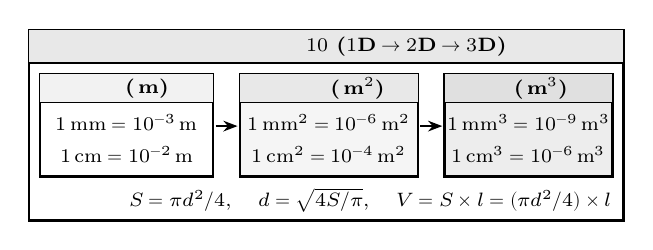
\begin{tikzpicture}[x=1cm, y=1cm, every node/.style={font=\scriptsize, text=black}]
  \draw[black, line width=0.9pt] (0,0) rectangle (7.55,2.42);
  \fill[gray!18] (0,2.00) rectangle (7.55,2.42);
  \draw[black, line width=0.6pt] (0,2.00) -- (7.55,2.00);
  \node at (3.775,2.21) {\textbf{ស្ពានបំប្លែងខ្នាតស្វ័យគុណគោល $10$ ($1\text{\en{D}} \to 2\text{\en{D}} \to 3\text{\en{D}}$)}};

  % Box 1: 1D
  \draw[black, line width=0.8pt] (0.14,0.56) rectangle (2.34,1.86);
  \fill[gray!10] (0.14,1.50) rectangle (2.34,1.86);
  \draw[black, line width=0.5pt] (0.14,1.50) -- (2.34,1.50);
  \node at (1.24,1.68) {\textbf{ប្រវែង ($\unit{m}$)}};
  \node at (1.24,1.24) {$1\unit{mm} = 10^{-3}\unit{m}$};
  \node at (1.24,0.84) {$1\unit{cm} = 10^{-2}\unit{m}$};

  \draw[-{Stealth[length=1.8mm]}, black, line width=0.8pt] (2.37,1.20) -- (2.65,1.20);

  % Box 2: 2D
  \draw[black, line width=0.85pt, fill=gray!8] (2.68,0.56) rectangle (4.94,1.86);
  \fill[gray!18] (2.68,1.50) rectangle (4.94,1.86);
  \draw[black, line width=0.5pt] (2.68,1.50) -- (4.94,1.50);
  \node at (3.81,1.68) {\textbf{ផ្ទៃក្រឡា ($\unit{m}^2$)}};
  \node at (3.81,1.24) {$1\unit{mm}^2 = 10^{-6}\unit{m}^2$};
  \node at (3.81,0.84) {$1\unit{cm}^2 = 10^{-4}\unit{m}^2$};

  \draw[-{Stealth[length=1.8mm]}, black, line width=0.8pt] (4.97,1.20) -- (5.25,1.20);

  % Box 3: 3D
  \draw[black, line width=0.95pt, fill=gray!14] (5.28,0.56) rectangle (7.41,1.86);
  \fill[gray!24] (5.28,1.50) rectangle (7.41,1.86);
  \draw[black, line width=0.55pt] (5.28,1.50) -- (7.41,1.50);
  \node at (6.345,1.68) {\textbf{មាឌ ($\unit{m}^3$)}};
  \node at (6.345,1.24) {$1\unit{mm}^3 = 10^{-9}\unit{m}^3$};
  \node at (6.345,0.84) {$1\unit{cm}^3 = 10^{-6}\unit{m}^3$};

  \node at (3.775,0.26) {រូបមន្តស៊ីឡាំង៖ $S = \pi d^2 / 4$, \quad $d = \sqrt{4S/\pi}$, \quad $V = S\times l = (\pi d^2 / 4)\times l$};
\end{tikzpicture}}

% ៤. E4 Elaborate: លំហាត់គំរូទី ២ (ទំ.៤៤ — ទាញរកអង្កត់ផ្ចិត d ពី S = \pi/4 x 10^{-6} m^2)
\newcommand{\figDiameterMEASFourOne}{%
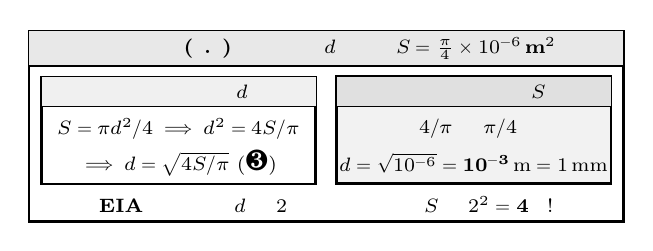
\begin{tikzpicture}[x=1cm, y=1cm, every node/.style={font=\scriptsize, text=black}]
  \draw[black, line width=0.9pt] (0,0) rectangle (7.55,2.42);
  \fill[gray!18] (0,1.98) rectangle (7.55,2.42);
  \draw[black, line width=0.6pt] (0,1.98) -- (7.55,1.98);
  \node at (3.775,2.20) {\textbf{លំហាត់គំរូទី ២ (ទំ.៤៤)៖ រកអង្កត់ផ្ចិត $d$ បើស្គាល់ $S = \frac{\pi}{4}\times 10^{-6}\unit{m}^2$}};

  \draw[black, line width=0.8pt] (0.16,0.48) rectangle (3.64,1.84);
  \fill[gray!12] (0.16,1.46) rectangle (3.64,1.84);
  \draw[black, line width=0.55pt] (0.16,1.46) -- (3.64,1.46);
  \node at (1.90,1.65) {\textbf{ជំហានទី ១៖ ទាញរូបមន្ត $d$}};
  \node at (1.90,1.18) {$S = \pi d^2 / 4 \implies d^2 = 4S/\pi$};
  \node at (1.90,0.74) {$\implies d = \sqrt{4S/\pi}$ (\cnum{3})};

  \draw[black, line width=0.95pt, fill=gray!10] (3.91,0.48) rectangle (7.39,1.84);
  \fill[gray!24] (3.91,1.46) rectangle (7.39,1.84);
  \draw[black, line width=0.6pt] (3.91,1.46) -- (7.39,1.46);
  \node at (5.65,1.65) {\textbf{ជំហានទី ២៖ ជំនួសតម្លៃ $S$}};
  \node at (5.65,1.18) {សម្រួល $4/\pi$ និង $\pi/4$ ក្រោមឫស៖};
  \node at (5.65,0.74) {$d = \sqrt{10^{-6}} = \mathbf{10^{-3}\unit{m}} = 1\unit{mm}$};

  \node at (3.775,0.22) {\textbf{\en{EIA}៖} បើអង្កត់ផ្ចិត $d$ កើន $2$ ដង នោះផ្ទៃក្រឡាមុខកាត់ $S$ កើន $2^2 = \mathbf{4}$ ដង!};
\end{tikzpicture}}

% ៥. E5 Evaluate: ជម្រើសវិនិច្ឆ័យ A-D (សរសៃដែកសាងសង់អង្កត់ផ្ចិត d = 10 mm គិតផ្ទៃមុខកាត់ជា m^2)
\newcommand{\figExitMEASFourOne}{%
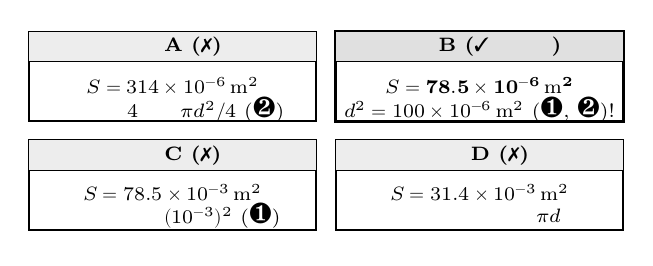
\begin{tikzpicture}[x=1cm, y=1cm, every node/.style={font=\scriptsize, text=black}]
  % Choice A
  \draw[black, line width=0.8pt] (0,1.38) rectangle (3.65,2.52);
  \fill[gray!14] (0,2.14) rectangle (3.65,2.52);
  \draw[black, line width=0.5pt] (0,2.14) -- (3.65,2.14);
  \node at (1.825,2.33) {\textbf{ជម្រើស \en{A} (\ding{55})}};
  \node at (1.825,1.84) {$S = 314\times 10^{-6}\unit{m}^2$};
  \node at (1.825,1.53) {ភ្លេចចែកនឹង $4$ ក្នុង $\pi d^2 / 4$ (\cnum{2})};

  % Choice B (Correct)
  \draw[black, line width=1.05pt] (3.90,1.38) rectangle (7.55,2.52);
  \fill[gray!24] (3.90,2.14) rectangle (7.55,2.52);
  \draw[black, line width=0.6pt] (3.90,2.14) -- (7.55,2.14);
  \node at (5.725,2.33) {\textbf{ជម្រើស \en{B} (\ding{51} ត្រឹមត្រូវ)}};
  \node at (5.725,1.84) {$S = \mathbf{78.5\times 10^{-6}\unit{m}^2}$};
  \node at (5.725,1.53) {$d^2 = 100\times 10^{-6}\unit{m}^2$ (\cnum{1}, \cnum{2})!};

  % Choice C
  \draw[black, line width=0.8pt] (0,0) rectangle (3.65,1.14);
  \fill[gray!14] (0,0.76) rectangle (3.65,1.14);
  \draw[black, line width=0.5pt] (0,0.76) -- (3.65,0.76);
  \node at (1.825,0.95) {\textbf{ជម្រើស \en{C} (\ding{55})}};
  \node at (1.825,0.48) {$S = 78.5\times 10^{-3}\unit{m}^2$};
  \node at (1.825,0.18) {ភ្លេចលើកការេខ្នាត $(10^{-3})^2$ (\cnum{1})};

  % Choice D
  \draw[black, line width=0.8pt] (3.90,0) rectangle (7.55,1.14);
  \fill[gray!14] (3.90,0.76) rectangle (7.55,1.14);
  \draw[black, line width=0.5pt] (3.90,0.76) -- (7.55,0.76);
  \node at (5.725,0.95) {\textbf{ជម្រើស \en{D} (\ding{55})}};
  \node at (5.725,0.48) {$S = 31.4\times 10^{-3}\unit{m}^2$};
  \node at (5.725,0.18) {ច្រឡំប្រើរូបមន្តបរិមាត្រ $\pi d$};
\end{tikzpicture}}

\begin{document}
\fontsize{10pt}{15.2pt}\selectfont

% ============================================================================
% ក្បាលរដ្ឋបាល (Administrative Header — តាមគំរូ ls_plan.tex)
% ============================================================================
{\centering
  {\muol\fontsize{11pt}{16pt}\selectfont ព្រះរាជាណាចក្រកម្ពុជា\par}
  {\muol\fontsize{11pt}{16pt}\selectfont ជាតិ សាសនា ព្រះមហាក្សត្រ\par}
  \vspace{-3pt}{\khmflourish\par}
}

\vspace{1pt}
{\muol\fontsize{10pt}{15.5pt}\selectfont
មន្ទីរអប់រំ យុវជន និងកីឡា ខេត្តកំពង់ធំ\par
ការិយាល័យអប់រំ យុវជន និងកីឡា ស្រុកកំពង់ស្វាយ\par
អនុវិទ្យាល័យព្រះក្រសាំង\par}

\vspace{4pt}
{\centering{\muol\fontsize{11.5pt}{17pt}\selectfont កិច្ចតែងការបង្រៀន\par}}
\vspace{3pt}

% --- ព័ត៌មានទូទៅ ---
{\hspace*{2.8cm}\renewcommand{\arraystretch}{1.08}
\begin{tabular}{@{}l@{\hspace{0.35cm}}p{2.9cm}@{\hspace{0.15cm}}c@{\hspace{0.25cm}}l@{}}
  - & មុខវិជ្ជា & : & គណិតវិទ្យា ថ្នាក់ទី៨ (ពីជគណិត) \\
  - & ចំណងជើងមេរៀន & : & មេរៀនទី៤៖ រង្វាស់រង្វាល់ \\
  - & ចំណងជើងរង & : & ១. ផ្ទៃក្រឡានិងមាឌ (ទំ.៤៣--៤៤, ៥០) \\
  - & រយៈពេល & : & ១ ម៉ោងសិក្សា (៥០ នាទី) \\
  - & បង្រៀនដោយ & : & ហុក ប៊ុនថែន \\
  - & កាលបរិច្ឆេទ & : & ថ្ងៃចន្ទ ទី៣០ ខែវិច្ឆិកា ឆ្នាំ២០២៦ \\
\end{tabular}\par}

\vspace{4pt}

% --- I. វត្ថុបំណង ---
{\muol\fontsize{10pt}{15.5pt}\selectfont \enbf{I.} វត្ថុបំណង\par}
\vspace{1pt}
{\renewcommand{\arraystretch}{1.10}
\begin{tabular}{@{}p{0.55cm}@{}p{2.35cm}@{\hspace{0.15cm}}c@{\hspace{0.25cm}}p{14.95cm}@{}}
  \hfill\wcirc\hspace{0.2cm} & វិជ្ជាសម្បទា & : & សិស្សប្រាប់ទំនាក់ទំនងបំប្លែងខ្នាតប្រវែងតូចៗ ($\unit{mm}, \unit{cm}, \unit{dm}$) ជាម៉ែត្រ ($\unit{m}$) តាមស្វ័យគុណគោល $10$ ព្រមទាំងរូបមន្តផ្ទៃក្រឡាមុខកាត់រាងរង្វង់ $S = \frac{\pi d^2}{4}$ និងមាឌស៊ីឡាំង $V = \frac{\pi d^2}{4}\times l$ គិតជា $\unit{m}^2$ និង $\unit{m}^3$ បានត្រឹមត្រូវ ។ \\
  \hfill\wcirc\hspace{0.2cm} & បំណិនសម្បទា & : & សិស្សគណនាផ្ទៃក្រឡាមុខកាត់ អង្កត់ផ្ចិត និងមាឌនៃវត្ថុដែលមានវិមាត្រតូចៗ (ខ្សែភ្លើង សរសៃដែកសាងសង់ និងឈើជ្រុង) គិតជា $\unit{m}^2$ និង $\unit{m}^3$ តាមតារាងស្ពានស្វ័យគុណគោល $10$ លើសន្លឹកកិច្ចការ (ទំ.៤៣--៤៤) បានត្រឹមត្រូវ ។ \\
  \hfill\wcirc\hspace{0.2cm} & ចរិយាសម្បទា & : & សិស្សមានទម្លាប់ត្រួតពិនិត្យនិងបំប្លែងខ្នាតរង្វាស់ឱ្យឯកភាពគ្នាជាម៉ែត្រ ($\unit{m}$) មុនជំនួសចូលរូបមន្តគណនាផ្ទៃក្រឡានិងមាឌសម្ភារៈប្រើប្រាស់ក្នុងជីវភាពរស់នៅប្រកបដោយភាពម៉ត់ចត់ ។ \\
\end{tabular}\par}

\vspace{3pt}

% --- II. សម្ភារៈឧបទេស ---
{\muol\fontsize{10pt}{15.5pt}\selectfont \enbf{II.} សម្ភារៈឧបទេស\par}
\vspace{1pt}
\hspace*{0.55cm}$\bullet$\ សៀវភៅសិក្សាគោលថ្នាក់ទី៨ (ទំ.៤៣--៤៤, ៥០) ក្ដារខៀន ដីស/ហ្វឺត បន្ទាត់ត្រង់ និង\textbf{សន្លឹកកិច្ចការសិស្សបំពេញចន្លោះ ស-ខ្មៅ} (\en{Printable\_Materials\_MEAS41} ទំព័រ ១--២ សម្រាប់សិស្ស និងទំព័រ ៣ ប្លង់ក្ដារខៀន/ចម្លើយគ្រូ — គ្មានប្រើ \en{LCD})\par

\vspace{3pt}

% --- III. វិធីសាស្រ្តបង្រៀន ---
{\muol\fontsize{10pt}{15.5pt}\selectfont \enbf{III.} វិធីសាស្រ្តបង្រៀន\par}
\vspace{1pt}
{\renewcommand{\arraystretch}{1.08}
\begin{tabular}{@{}p{0.55cm}@{}p{2.35cm}@{\hspace{0.15cm}}c@{\hspace{0.25cm}}p{14.95cm}@{}}
  \hfill$\bullet$\hspace{0.2cm} & គោលវិធី & : & សិស្សមជ្ឈមណ្ឌល (សន្លឹកកិច្ចការបំពេញចន្លោះជាគោល + ការពិភាក្សាជាក្រុមតូច ៣ នាក់) \\
  \hfill$\bullet$\hspace{0.2cm} & យុទ្ធវិធីបង្រៀន & : & គំរូស្ថាបនានិយម \en{5Es} រួមបញ្ចូល \textbf{ស្ពានស្វ័យគុណគោល ១០ ($1\text{\en{D}} \to 2\text{\en{D}} \to 3\text{\en{D}}$)} និង \textbf{ការវិភាគវិមាត្រមុនជំនួសរូបមន្ត} \\
\end{tabular}\par}

\vspace{3pt}

% --- IV. ដំណើរការបង្រៀន ---
{\muol\fontsize{10pt}{15.5pt}\selectfont \enbf{IV.} ដំណើរការបង្រៀន\par}

{\renewcommand{\arraystretch}{1.15}
\begin{longtable}{|L{5.50cm}|L{7.90cm}|L{4.80cm}|}
\hline
\multicolumn{1}{|c|}{\cellcolor{headgray}\muol សកម្មភាពគ្រូ} &
\multicolumn{1}{c|}{\cellcolor{headgray}\muol ខ្លឹមសារមេរៀន} &
\multicolumn{1}{c|}{\cellcolor{headgray}\muol សកម្មភាពសិស្ស} \\
\hline
\endfirsthead

\hline
\multicolumn{1}{|c|}{\cellcolor{headgray}\muol សកម្មភាពគ្រូ} &
\multicolumn{1}{c|}{\cellcolor{headgray}\muol ខ្លឹមសារមេរៀន} &
\multicolumn{1}{c|}{\cellcolor{headgray}\muol សកម្មភាពសិស្ស} \\
\hline
\endhead

% ==================== ជំហានទី១ (2min) ====================
\stepheader{ជំហានទី១ \enbf{(}រដ្ឋបាលថ្នាក់\enbf{)}}
$\bullet$ ពិនិត្យវត្តមាន អនាម័យ និងសណ្ដាប់ធ្នាប់ថ្នាក់រៀន \par
$\bullet$ រៀបចំក្រុមតូច ៣ នាក់តាមតុ និងចែក\textbf{សន្លឹកកិច្ចការសិស្ស (\en{MEAS41} ទំព័រ ១–២)}
&
$\bullet$ រដ្ឋបាលថ្នាក់ អនាម័យ និងវិន័យសិក្សា \par
$\bullet$ ចែកសន្លឹកកិច្ចការម្នាក់ ១ សន្លឹក សម្រាប់បំពេញតាមដំណាក់កាល \en{E1--E5}
&
$\circ$ ប្រធានថ្នាក់រាយការណ៍វត្តមានសិស្ស \par
$\circ$ ទទួលសន្លឹកកិច្ចការ សរសេរឈ្មោះ និងអង្គុយតាមក្រុម ៣ នាក់ \\
\hline

% ==================== ជំហានទី២ (9min: កំណែ <=3m + រំលឹក 3m + E1 3m) ====================
\stepheader{ជំហានទី២ \enbf{(}កិច្ចការផ្ទះ \enbf{+} ទំនាក់ទំនងមេរៀនថ្មី\enbf{)}}
\ditem \textbf{កំណែកិច្ចការផ្ទះ ($\le\text{\enbf{3\,min}}$)} \par
$\bullet$ ហៅសិស្ស ២ នាក់ឡើងកែលំហាត់ទំ.៤២ លេខ ១៩(ក, ខ) លើក្ដារខៀន
&
{\centering\redsub{កំណែកិច្ចការផ្ទះមេរៀនមុន (ទំ.៤២ \#19 ក និង ខ)}\par}
$\bullet$ \textbf{\#19 (ទំ.៤២ — ពូគាទិញម៉ាស៊ីនត្រជាក់ $2\,700\,000\riel$, កក់ $20\%$, $48$ ខែ, $10\%$/ឆ្នាំ)៖} \par
\hspace*{0.2cm}-- $D = 540\,000\riel, B = 2\,160\,000\riel, I = 864\,000\riel \implies S = 3\,024\,000\riel$ \par
\hspace*{0.2cm}-- \textbf{(ក)} សងប្រចាំខែ $M = \mathbf{63\,000\riel}$/ខែ; \ \textbf{(ខ)} សន្សំបាន $\mathbf{864\,000\riel}$
&
$\circ$ ផ្ទៀងចម្លើយ និងកែតម្រូវចូលសៀវភៅកិច្ចការផ្ទះ \\[3pt]

\ditem \textbf{រំលឹកមេរៀនទាក់ទង (\enbf{3min})} \par
$\bullet$ សួរ៖ «តើ $\frac{1}{1\,000}$ សរសេរជាស្វ័យគុណគោល $10$ ដូចម្ដេច? ចុះ $(10^{-3})^2$ ស្មើប៉ុន្មាន?»
&
{\centering\redsub{រំលឹកស្វ័យគុណគោល $10$ និងផ្ទៃក្រឡារង្វង់}\par}
$\bullet$ ស្វ័យគុណគោល $10$៖ $0.001 = \tfrac{1}{1\,000} = 10^{-3}$ និង $(10^{-3})^2 = 10^{-6}$
&
$\circ$ ឆ្លើយ៖ «$0.001 = 10^{-3}$ ហើយ $(10^{-3})^2 = 10^{-6}$!» \\[3pt]

$\bullet$ សួរបន្ត៖ «បើរង្វង់មានអង្កត់ផ្ចិត $d$ ($r = \frac{d}{2}$) តើផ្ទៃក្រឡា $S = \pi r^2$ សរសេរតាម $d$ ដូចម្ដេច?»
&
$\bullet$ ផ្ទៃរង្វង់ស្គាល់អង្កត់ផ្ចិត $d$៖ $S = \pi\left(\tfrac{d}{2}\right)^2 = \pi\times \dfrac{d^2}{4}$ ($\pi \approx 3.14$)
&
$\circ$ ឆ្លើយ៖ «$S = \pi\times \frac{d^2}{4}$!» \\[3pt]

\fiveE{E1 - Engage (3min)} \timenote{(កុំទាន់ផ្ដល់ចម្លើយ)} \par
\ditem \textbf{បេសកកម្មជាងអគ្គិសនីវាស់មុខកាត់តូច (សន្លឹកកិច្ចការ \en{E1})} \par
$\bullet$ ឱ្យសិស្សអានប្រអប់ \en{E1} ហើយគូសជ្រើសរើសរវាង\textbf{កូនជាងទី ១} និង\textbf{កូនជាងទី ២}
&
\redsub{បេសកកម្ម \en{E1}៖ ការេតូចមានជ្រុង $1\unit{mm} = 10^{-3}\unit{m}$ តើផ្ទៃក្រឡាស្មើប៉ុន្មាន $\unit{m}^2$?} \par
ជាងអគ្គិសនីពិនិត្យបន្ទះលោហៈរាងការេតូចមួយមានជ្រុង $a = 1\unit{mm} = 10^{-3}\unit{m}$ ។ \par
$\bullet$ កូនជាងទី ១ ថា $S = 10^{-3}\unit{m}^2$ រីឯកូនជាងទី ២ ថា $S = 10^{-6}\unit{m}^2$ ។ តើអ្នកណាត្រូវ?
&
$\circ$ ពិភាក្សាជាគូ និងគូស \ding{51} ក្នុងប្រអប់ \en{E1} លើសន្លឹកកិច្ចការ \\[3pt]

&
\cfig{\figEngageMEASFourOne}
& \\
\hline

% ==================== ជំហានទី៣ (17min: E2 11m + E3 6m) ====================
\stepheader{ជំហានទី៣ \enbf{(}ខ្លឹមសារមេរៀនថ្មី\enbf{)}}
\fiveE{E2 - Explore (11min)} \par
$\bullet$ សរសេរចំណងជើង \textbf{មេរៀនទី៤៖ រង្វាស់រង្វាល់ — ១. ផ្ទៃក្រឡានិងមាឌ} លើក្ដារខៀន \par
\ditem \textbf{សកម្មភាព ១៖ បំប្លែងខ្នាតតូច និងលំហាត់គំរូទី ១ (\enbf{6min}, សន្លឹកកិច្ចការ \en{E2-A})} \par
$\bullet$ ឱ្យសិស្សបំពេញប្រអប់បំប្លែងខ្នាត (ទំ.៤៣) រួចគណនាផ្ទៃមុខកាត់ខ្សែភ្លើង $d = 2\unit{mm}$
&
មេរៀនទី៤ \quad {\muol រង្វាស់រង្វាល់} \par
១. ផ្ទៃក្រឡានិងមាឌ \par
$\bullet$ \textbf{បំប្លែងខ្នាតប្រវែងជាម៉ែត្រ (ទំ.៤៣)៖} $1\unit{mm} = 10^{-3}\unit{m}, \ 1\unit{cm} = 10^{-2}\unit{m}, \ 1\unit{dm} = 10^{-1}\unit{m}$ \par
$\bullet$ \textbf{លំហាត់គំរូទី ១ (ទំ.៤៣–៤៤ — ខ្សែភ្លើងរាងស៊ីឡាំង $d = 2\unit{mm}, \pi = 3.14$)៖} \par
\hspace*{0.2cm}-- បំប្លែងអង្កត់ផ្ចិត៖ $d = 2\unit{mm} = 2\times 10^{-3}\unit{m} \implies d^2 = (2\times 10^{-3}\unit{m})^2 = \mathbf{4\times 10^{-6}\unit{m}^2}$ \par
\hspace*{0.2cm}-- ផ្ទៃក្រឡាមុខកាត់៖ $S = \pi\times \dfrac{d^2}{4} = 3.14\times \dfrac{4\times 10^{-6}}{4} = 3.14\times 10^{-6}\unit{m}^2 = \mathbf{314\times 10^{-8}\unit{m}^2}$
&
$\circ$ បំប្លែង $d = 2\times 10^{-3}\unit{m}$ លើកការេ និងគណនាឃើញ $S = 314\times 10^{-8}\unit{m}^2$ \\[3pt]

&
\cfig{\figWireCrossMEASFourOne}
& \\[3pt]

\ditem \textbf{សកម្មភាព ២៖ អន្ទាក់ភ្លេចលើកការេខ្នាត និងភ្លេចចែកនឹង $4$ (\enbf{5min}, សន្លឹកកិច្ចការ \en{E2-B})} \par
$\bullet$ សួរ៖ «ហេតុអ្វី $d^2$ មានខ្នាត $10^{-6}\unit{m}^2$ មិនមែន $10^{-3}\unit{m}^2$? ចុះបើភ្លេចចែកនឹង $4$ ខុសប៉ុន្មានដង?»
&
$\bullet$ \textbf{ពិនិត្យអន្ទាក់ទាំងពីរ៖} \par
\hspace*{0.2cm}-- \textbf{អន្ទាក់ទី ១ (ខ្នាត)៖} $(2\times 10^{-3}\unit{m})^2 = 2^2 \times (10^{-3})^2\unit{m}^2 = 4\times 10^{-6}\unit{m}^2$ (បើដាក់ $10^{-3}$ ខុស $1\,000$ ដង!) \par
\hspace*{0.2cm}-- \textbf{អន្ទាក់ទី ២ (អង្កត់ផ្ចិត $d$ ទល់នឹងកាំ $r$)៖} បើសរសេរ $\pi d^2$ ដោយភ្លេចចែកនឹង $4$ លទ្ធផលធំជាងការពិត $4$ ដង! \par
\hspace*{0.2cm}-- ចំពោះមាឌ $1\unit{cm}^3 = (10^{-2}\unit{m})^3 = \mathbf{10^{-6}\unit{m}^3}$ និងមាឌស៊ីឡាំង $V = S\times l$
&
$\circ$ រកឃើញថាត្រូវបំប្លែងជា $\unit{m}$ មុនលើកការេ និងត្រូវចែក $d^2$ នឹង $4$ ជានិច្ច \\[3pt]

% --- E3 Explain (6min) ---
\fiveE{E3 - Explain (6min)} \par
$\bullet$ ដឹកនាំសិស្សសង្ខេបតារាងបំប្លែងខ្នាត និងរូបមន្តផ្ទៃក្រឡា-មាឌ (ទំ.៤៣–៤៤)
&
$\bullet$ \textbf{សង្ខេបរូបមន្តបំប្លែងខ្នាត ផ្ទៃក្រឡា និងមាឌ (ទំ.៤៣–៤៤)៖} \par
\hspace*{0.15cm}១) ប្រវែង៖ \graybox{$1\unit{mm} = 10^{-3}\unit{m}$} \quad \graybox{$1\unit{cm} = 10^{-2}\unit{m}$} \quad \graybox{$1\unit{dm} = 10^{-1}\unit{m}$}
&
$\circ$ បំពេញប្រអប់ខ្នាតប្រវែងលើសន្លឹកកិច្ចការ \en{E3} \\[3pt]

$\bullet$ កត់ត្រារូបមន្តផ្ទៃមុខកាត់ស៊ីឡាំង អង្កត់ផ្ចិត និងមាឌស៊ីឡាំង/ប្រលេពីប៉ែតកែង
&
\hspace*{0.15cm}២) មុខកាត់រង្វង់៖ \graybox{$S = \dfrac{\pi d^2}{4}$} \quad ទាញរកអង្កត់ផ្ចិត៖ \graybox{$d = \sqrt{\dfrac{4S}{\pi}}$} \quad មាឌ៖ \graybox{$V = S\times l = \dfrac{\pi d^2}{4}\times l$}
&
$\circ$ កត់ត្រារូបមន្ត $S, d$ និង $V$ លើសន្លឹកកិច្ចការ \en{E3} \\[3pt]

&
\cfig{\figBridgeMEASFourOne}
& \\[3pt]

$\bullet$ ភ្ជាប់\textbf{ធនាគារហេតុផល \cnum{1}--\cnum{4}} លើក្ដារខៀន និងសន្លឹកកិច្ចការ
&
\textbf{ធនាគារហេតុផល (\en{Warrant Bank})៖} \par
\cnum{1} \textbf{បំប្លែងជា $\unit{m}$ មុនជំនួស៖} $1\unit{mm} = 10^{-3}\unit{m} \implies 1\unit{mm}^2 = 10^{-6}\unit{m}^2$; $1\unit{cm} = 10^{-2}\unit{m} \implies 1\unit{cm}^2 = 10^{-4}\unit{m}^2$ \par
\cnum{2} \textbf{ផ្ទៃមុខកាត់តាមអង្កត់ផ្ចិត៖} $S = \frac{\pi d^2}{4}$ (កុំភ្លេចចែកនឹង $4$!) \par
\cnum{3} \textbf{ទាញរកអង្កត់ផ្ចិត $d$៖} $d = \sqrt{\frac{4S}{\pi}}$ ($S$ គិតជា $\unit{m}^2 \implies d$ គិតជា $\unit{m}$) \par
\cnum{4} \textbf{មាឌវត្ថុមុខកាត់ស្មើ៖} $V = S\times l$ (ស៊ីឡាំង $V = \frac{\pi d^2}{4}\times l$; ឈើជ្រុង $V = a\times b\times l$ គិតជា $\unit{m}^3$)
&
$\circ$ ផ្ទៀងលេខកូដ \cnum{1}--\cnum{4} លើសន្លឹកកិច្ចការ \\
\hline

% ==================== ជំហានទី៤ (20min: E4 10m + E5 10m) ====================
\stepheader{ជំហានទី៤ \enbf{(}ពង្រីកចំណេះដឹង\enbf{)}}
\fiveE{E4 - Elaborate (10min)} \par
\ditem \textbf{លំហាត់គំរូទី ២៖ គណនាអង្កត់ផ្ចិតខ្សែភ្លើងពីផ្ទៃក្រឡាមុខកាត់ (ទំ.៤៤)} \par
$\bullet$ ឱ្យសិស្សបំពេញជំហានទាញរូបមន្ត និងជំនួស $S = \frac{\pi}{4}\times 10^{-6}\unit{m}^2$ លើសន្លឹកកិច្ចការ \en{E4}
&
{\muol លំហាត់គំរូទី ២} \textbf{(ទំ.៤៤ — គណនាអង្កត់ផ្ចិតខ្សែភ្លើង បើ $S = \frac{\pi}{4}\times 10^{-6}\unit{m}^2$)៖} \par
$\bullet$ តាមរូបមន្ត $S = \dfrac{\pi d^2}{4} \implies d^2 = \dfrac{4S}{\pi} \implies d = \sqrt{\dfrac{4S}{\pi}}$ (\cnum{3}) \par
$\bullet$ ជំនួសតម្លៃ $S = \dfrac{\pi\times 10^{-6}}{4}$៖ \quad $d = \sqrt{\dfrac{4}{\pi}\times \dfrac{\pi\times 10^{-6}}{4}} = \sqrt{10^{-6}} = \graybox{$10^{-3}\unit{m}$} = 1\unit{mm}$ \par
$\bullet$ \textbf{ពង្រីកភ្ជាប់ឈើជ្រុង៖} បើឈើជ្រុងមានមុខកាត់ $4\unit{cm}\times 8\unit{cm}$ ប្រវែង $5\unit{m}$ $\implies V = 0.04\times 0.08\times 5 = \mathbf{0.016\unit{m}^3}$ (\cnum{4})
&
$\circ$ សម្រួល $\pi$ និង $4$ ក្រោមឫសការេ រកឃើញ $d = 10^{-3}\unit{m}$ និងមាឌឈើជ្រុង $0.016\unit{m}^3$ \\[3pt]

&
\cfig{\figDiameterMEASFourOne}
& \\[3pt]

$\bullet$ សួរសំណួរឆ្លុះបញ្ចាំង \textbf{\en{EIA Looking-Back} (1min)}
&
\textbf{\en{EIA Looking-Back}៖} «បើអង្កត់ផ្ចិតខ្សែភ្លើងកើនឡើង $2$ ដង (ពី $1\unit{mm}$ ទៅ $2\unit{mm}$) តើផ្ទៃក្រឡាមុខកាត់ $S$ កើនប៉ុន្មានដង?» ($\to$ កើន $2^2 = \mathbf{4}$ ដង ព្រោះក្នុងរូបមន្តមាន $d^2$!)
&
$\circ$ ឆ្លើយថាផ្ទៃក្រឡាកើន $4$ ដង ដោយសារ $d$ លើកជាការេ \\[3pt]

% --- E5 Evaluate (10min) ---
\fiveE{E5 - Evaluate (10min)} \par
\ditem \textbf{ប្រតិបត្តិជាក្រុមតូច ៣ នាក់ (4min, សន្លឹកកិច្ចការ \en{E5})} \par
$\bullet$ ឱ្យសិស្សគណនាមាឌខ្សែភ្លើង $d = 2\unit{cm}, l = 200\unit{m}$ (ទំ.៤៤) តាមធនាគារហេតុផល \cnum{1}, \cnum{2}, \cnum{4}
&
{\muol លំហាត់ប្រតិបត្តិ} \textbf{(ទំ.៤៤ — រកមាឌខ្សែភ្លើងអង្កត់ផ្ចិត $d = 2\unit{cm}$, ប្រវែង $l = 200\unit{m}, \pi = 3.14$)៖} \par
$\bullet$ បំប្លែងខ្នាត៖ $d = 2\unit{cm} = 2\times 10^{-2}\unit{m} \implies d^2 = 4\times 10^{-4}\unit{m}^2$ (\cnum{1}) \par
$\bullet$ ផ្ទៃមុខកាត់៖ $S = 3.14\times \dfrac{4\times 10^{-4}}{4} = 3.14\times 10^{-4}\unit{m}^2$ (\cnum{2}) \par
$\bullet$ មាឌខ្សែភ្លើង៖ $V = S\times l = 3.14\times 10^{-4}\times 200 = 628\times 10^{-4}\unit{m}^3 = \graybox{$6.28\times 10^{-2}\unit{m}^3$} = 0.0628\unit{m}^3$ (\cnum{4})
&
$\circ$ គណនាជាក្រុមឃើញ $V = 6.28\times 10^{-2}\unit{m}^3$ ($0.0628\unit{m}^3$) \\[3pt]

$\bullet$ ឱ្យក្រុមសិស្សផ្ទៀងផ្ទាត់និង\textbf{បិទបេសកកម្ម \en{E1} (2min)}
&
$\bullet$ \textbf{បិទបេសកកម្ម \en{E1}៖} កូនជាងទី ២ ត្រឹមត្រូវ! ការេជ្រុង $1\unit{mm} = 10^{-3}\unit{m}$ មានផ្ទៃក្រឡា $S = (10^{-3}\unit{m})^2 = \mathbf{10^{-6}\unit{m}^2}$ (តូចជាង $10^{-3}\unit{m}^2$ ចំនួន $1\,000$ ដង!) ។
&
$\circ$ បិទបេសកកម្ម \en{E1} ឃើញកូនជាងទី ២ ត្រឹមត្រូវ ($10^{-6}\unit{m}^2$) \\[3pt]

\ditem \textbf{សំណួរវិនិច្ឆ័យ \en{A--D} និងសំបុត្រចេញ (4min)} \par
$\bullet$ ឱ្យសិស្សគូសរង្វង់ជម្រើសត្រូវលើសន្លឹកកិច្ចការ រួចលើកម្រាមដៃ ១--៤
&
{\centering\textbf{សំណួរវិនិច្ឆ័យ \en{A--D}៖ សរសៃដែកសាងសង់មួយដើមមានអង្កត់ផ្ចិត $d = 10\unit{mm}$ ($\pi = 3.14$) ។ តើផ្ទៃក្រឡាមុខកាត់វាស្មើប៉ុន្មាន $\unit{m}^2$?}\par}
&
$\circ$ វិភាគជម្រើស \en{A--D} និងលើកម្រាមដៃ ២ (\textbf{ជម្រើស \en{B}}) \\[3pt]

&
\cfig{\figExitMEASFourOne}
& \\[3pt]

$\bullet$ បញ្ជាក់ចម្លើយត្រូវ (\textbf{ជម្រើស \en{B}}) និងឱ្យបំពេញ\textbf{សំបុត្រចេញ ៦០ វិនាទី}
&
$\bullet$ \textbf{សំបុត្រចេញ៖} ខ្សែភ្លើងអង្កត់ផ្ចិត $d = 4\unit{mm} = 4\times 10^{-3}\unit{m}$ និងប្រវែង $l = 100\unit{m}$ ($\pi = 3.14$) $\implies S = \mathbf{12.56\times 10^{-6}\unit{m}^2}$ និងមាឌ $V = \mathbf{1.256\times 10^{-3}\unit{m}^3}$ ។
&
$\circ$ បំពេញសំបុត្រចេញលើសន្លឹកកិច្ចការមុនបញ្ចប់ម៉ោង \\
\hline

% ==================== ជំហានទី៥ (<=2min) ====================
\stepheader{ជំហានទី៥ \enbf{(}កិច្ចការផ្ទះ \enbf{+} បណ្ដាំផ្ញើ\enbf{)}}
\timenote{ចំណាយពេលឱ្យតិចបំផុតកុំឱ្យលើស 2min} \par
$\bullet$ ណែនាំប្រអប់\textbf{កិច្ចការផ្ទះ}លើសន្លឹកកិច្ចការទំព័រ ២ (លំហាត់ទំ.៥០ លេខ ១ ក-គ, លេខ ២ ក និងលេខ ៣)
&
{\centering{\muol កិច្ចការផ្ទះ} \textbf{(សៀវភៅគោល ទំ.៥០ លេខ ១ ក,ខ,គ, លេខ ២ ក និងលេខ ៣)}\par} \par
$\bullet$ \textbf{\#1 (ក,ខ,គ)៖} ផ្ទៃមុខកាត់ស៊ីឡាំងគិតជា $\unit{m}^2$៖ (ក) $1.5\unit{mm}$; (ខ) $2.5\unit{mm}$; (គ) $0.2\unit{mm}$ \par
$\bullet$ \textbf{\#2 (ក)៖} មាឌសរសៃដែក $d = 6\unit{mm}, l = 12\unit{m}$; \quad \textbf{\#3៖} ថ្លៃឈើជ្រុង $50$ ដើម ($4\unit{cm}\times 8\unit{cm}, l = 4.5\unit{m}$, $1\unit{m}^3$ ថ្លៃ $1\,200\,000\riel$) ។
&
$\circ$ គូសចំណាំលំហាត់ \#1(ក,ខ,គ), \#2(ក) និង \#3 ទំ.៥០ \\[3pt]

$\bullet$ ផ្ដាំផ្ញើឱ្យអានមុនចំណុចទី ២ សម្រាប់ម៉ោងក្រោយ
&
$\bullet$ \textbf{បណ្ដាំផ្ញើ៖} អានមុន \textbf{២. ម៉ាសធៀបនឹងផ្ទៃក្រឡា (ទំ.៤៤–៤៦)} និងពិនិត្យក្របក្រដាសរ៉ាម $\unit{g/m}^2$ ។
&
$\circ$ កត់ត្រាបណ្ដាំផ្ញើ ទុកសន្លឹកកិច្ចការក្នុងសៀវភៅ និងជម្រាបលាគ្រូ \\
\hline
\end{longtable}}

\vspace{6pt}
% --- ហត្ថលេខា (កាលបរិច្ឆេទត្រូវគ្នា ១០០% នឹងខាងលើ) ---
{\centering
\hspace*{5.2cm}\begin{minipage}{11.5cm}
  \centering
  ថ្ងៃចន្ទ ៦រោច ខែកត្តិក ឆ្នាំមមី អដ្ឋស័ក ពុទ្ធសករាជ ២៥៧០\par
  កំពង់ស្វាយ, ថ្ងៃទី៣០ ខែវិច្ឆិកា ឆ្នាំ២០២៦\par
  \vspace{2pt}
  {\muol គ្រូបង្រៀន\par}
  \vspace{32pt}
  \hfill{\muol ហុក ប៊ុនថែន}\hspace*{1.4cm}
\end{minipage}\par}

\end{document}
